
%\section{Models}
%In order to estimate a dense depth map $\mathbf{Z}$ from an RGB image $I$ architectures like UNet \cite{UNet} or DispNet \cite{DispNet}, which is in turn based on FlowNet \cite{FlowNet}, are used.
%They have an encoder-decoder structure with long range skip connections to avoid information loss during the encoding phase. 
%Older works \cite{Eigen} \cite{Eigen2} use modified classification networks like AlexNet \cite{AlexNet} or VGG \cite{VGG} using fully connected layers as upsamplers, this limits the resulting depth map resolution considerably.
%\cite{ResNet} as encoder backbone is more common \cite{MonoDepth2}.
%
%Encoder-decoder models are made to work at multiple scales by mapping intermediate feature maps from the decoder to depth maps at various scales.
%During training multi-scale outputs can be weighted favouring coarse-scale learning in early training stages and finer-scale later during training like in \cite{DispNet}.
%These intermediate mappings are realised via a linear or convolutional layer, but some authors also used graph convolutional networks \cite{GCNDepth}.
%
%
%Different approaches can be used in order to obtain a meaningful output.
%The output can be obtained by a linear operation, in this case the output values can be positive or negative and the output can be naturally interpreted as a disparity value or as a log depth value, although also considering it as a depth value is done \cite{Eigen}.
%In \cite{SfMLearner} the following activation function is applied to the output of the network for obtaining a depth map:
%\[
%	\mathbf{Z} = \frac{1}{\alpha * \sigma(x) + \beta}
%\]
%Where $\sigma$ is the sigmoid activation function, $\alpha=10$ and $\beta=0.01$.
%The resulting output depth range is approximately $(0.01, 100)$.
%
%Transformers.
%Markov Random Field, Conditional Random Fields, Neural Conditional Random Fields.

\section{Datasets}
Deep learning models learn the data distribution fed to them.
For example, if a model always receives car images during its training phase, then when an image without a car is presented to it, it will likely behave as if there was a car in the middle of the image.
Hence, datasets characteristics must be described in order to understand the behavior of models trained on them, in particular their ability to \textit{transfer} their knowledge to unseen contexts.

From a depth estimation perspective, the geometry of a scene is majorly affected by whether it is indoor or outdoor.
Indoor images present a limited range of depth values, while in outdoor scenes this can get quite large or be not defined, e.g. in pixels corresponding to the sky.
These two kind of environments semantically differ by involving objects of generally different categories that are rarely found depicted together.
In an outdoor image buildings, cars, roads and traffic signs are common, while in an indoor one furniture, paintings and dresses can appear.

Illumination (day or night), resolution (HD, 4K, ...) and weather conditions (foggy, rainy, clear, ...) in which images were captured are other relevant factors.
We say that a model operates \textit{into the wild} if it has been trained on images of unstructured environments.
Datasets of such scenes are \cite{DIW} \cite{ReDWeb} \cite{Youtube3D}, but they are used for \textit{relative} depth estimation, i.e. knowing which pixels correspond to closer objects than others.

The main datasets historically used for benchmarking monocular depth estimation (DE) techniques are KITTI \cite{KITTI} and NYUv2 \cite{NYUv2}.
Although, due to the increasing computational power and availability of data, in recent years DE methods are being benchmarked on a lot of datasets in order to evaluate their zero-shot performance \cite{MiDas, PatchFusion, Marigold, ZoeDepth}.

The progress of computer graphics made also possible to create photorealistic synthetic dataset \textit{densely} annotated.
Depth information is expensive to acquire and there are technical challenges that make it impossible to measure depth values corresponding to every pixel of an image.
For instance, LIDAR sensors are not able to measure depth values in correspondence of reflective objects.
Kinect sensors are instead limited in the detectable depth range.
Synthetic datasets can overcome these difficulties, but rendered scenes are less complex than real world ones.
Transferability is an issue of models trained purely on synthetic data.
Marigold \cite{Marigold} empirically proved that it is possible to obtain SOTA performances in DE by just fine-tuning a pre-trained vision foundation model (adapted to DE) on synthetic datasets.
They used Virtual KITTI 2 \cite{VirtualKITTI2} and Hypersim \cite{Hypersim}, respectively created in 2020 and 2021.

Virtual KITTI 2 \cite{VirtualKITTI2} is a synthetic version of the KITTI dataset\footnote{The "2" represents the version of the virtual dataset, Virtual KITTI "1" was created in 2016.} produced with the Unity game engine.
Originally, it was a virtual reproduction of the driving scenes from KITTI, but later more features wwere added.
It now contains annotated driving sequences captured in various weather and lighting conditions.

Hypersim \cite{Hypersim} is an indoor photorealistic synthetic dataset from Apple.
To create the dataset, they use publicly available 3D scenes produced by professional artists.
The dataset targets the general scene understanding task, making available various kinds of annotations (depth, illumination, semantic segmentation, 3D object detection and others).
The authors developed a cloud pipeline that sample camera view points from each scene and render various images under different lighting settings.
The procedure is illustrated in \cite{Hypersim} and allows also for dynamic interactive labeling of the meshes.

There are many other datasets that providing depth information \cite{Cityscapes, saxena5, ETH, DIODE, SYNTHIA, DispNet}.
See also \cite{MiDas} for an additional list, but they won't be treated here.
The following subsections are dedicated to the KITTI and NYUv2 datasets.

\subsection{KITTI}
Developing autonomous systems that are able to assist humans in everyday tasks is one of the grand challenges in modern computer science \cite{KITTI}.
The KITTI dataset \cite{KITTI} provides annotated data usable for such purpose (Figure \ref{fig:kitti_example}).
It consists of annotated images captured by a car mounting various sensors.
A stereo-rig with two pairs of cameras capture both colored and gray images (the latter with higher resolution).
A Velodyne (LIDAR) sensor measures depth values producing a point cloud that is projected onto the captured images, obtaining sparse ground truth depth maps.
Finally, also a GPS/IMU localization unit is used for tracking the car route.
The overall setup is illustrated in figure \ref{fig:kitti_car}.

\begin{figure}
	\begin{adjustwidth}{-0.2\textwidth}{-0.2\textwidth}
	\centering
    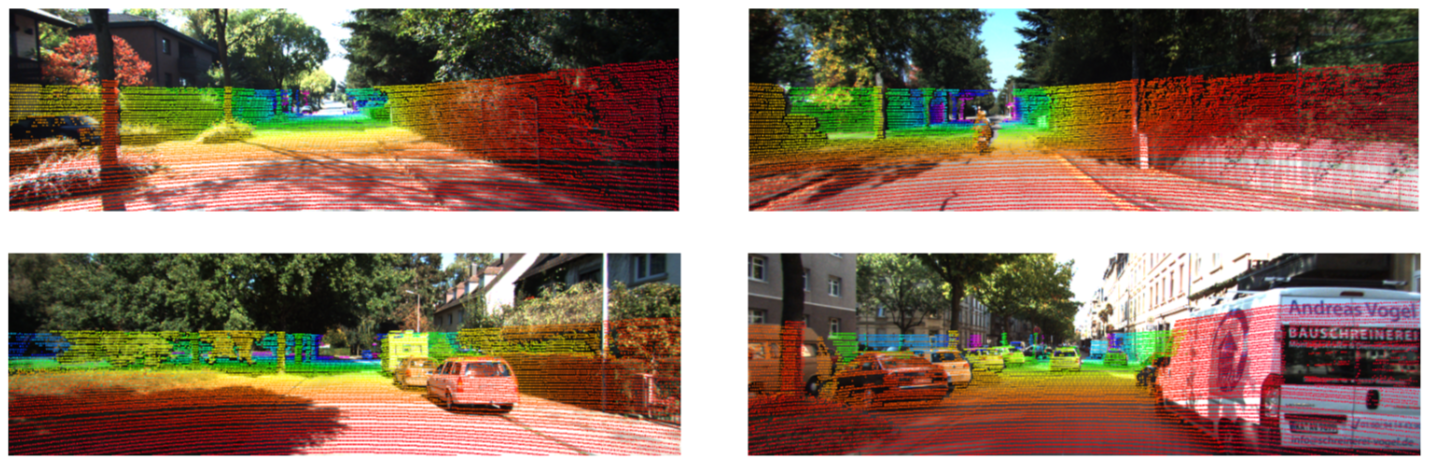
\includegraphics[width=\textwidth]{figs/kitti_example_2}
	\end{adjustwidth}
    \caption[Examples from the KITTI dataset.]{
        Images from KITTI and their ground-truth sparse depth maps.
        \label{fig:kitti_example}
    }
\end{figure}

Along various driving sessions, the car records data from all the sensors which are then cleaned and temporally aligned.
The dataset is hence organized as annotated video footage from the various sessions counting more than 40.000 images.
The driving sessions are all outdoor and with daylight illumination conditions.
Before each driving session a calibration phase is conducted.
All calibration information are available in the dataset, this includes also stereo baseline and camera parameters.
For this reason, the dataset is particularly suitable to self-supervised training that exploit geometrical constraints of cameras.
All the self-supervised works that will be reviewed in this thesis use this same dataset.
Other than depth maps, various kind of annotations are provided.
Parts of the dataset have been subsequently annotated for tasks such as object detection, image segmentation, optical flow estimation and others.
In here, depth data is the focus, but there are works tackling depth estimation by learning multiple tasks at once (e.g. image segmentation and depth estimation).
These are not treated here, some of them are discussed in \cite{MERTAN2022103441}.

\begin{figure}
	\centering
    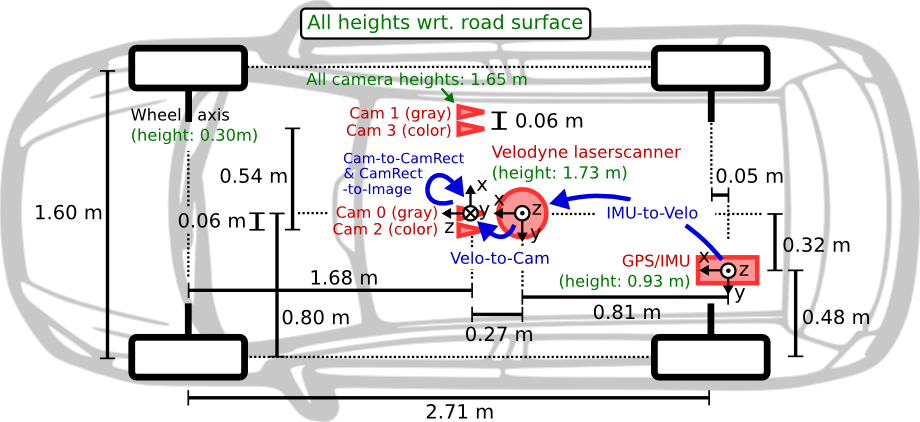
\includegraphics[width=0.8\textwidth]{figs/kitti_car}
    \caption[Car setup used for collecting KITTI data.]{
        Car setup used for acquiring KITTI data \cite{KITTI}, the image is from their website.
        \label{fig:kitti_car}
    }
\end{figure}
%%%%%%%%%%%%%%%%%%%%%%%%%%%%%%%%%%%%%%%%%%
% TODO: use sparsely annotated depth maps, not completed ones.

\begin{figure}
	\centering
    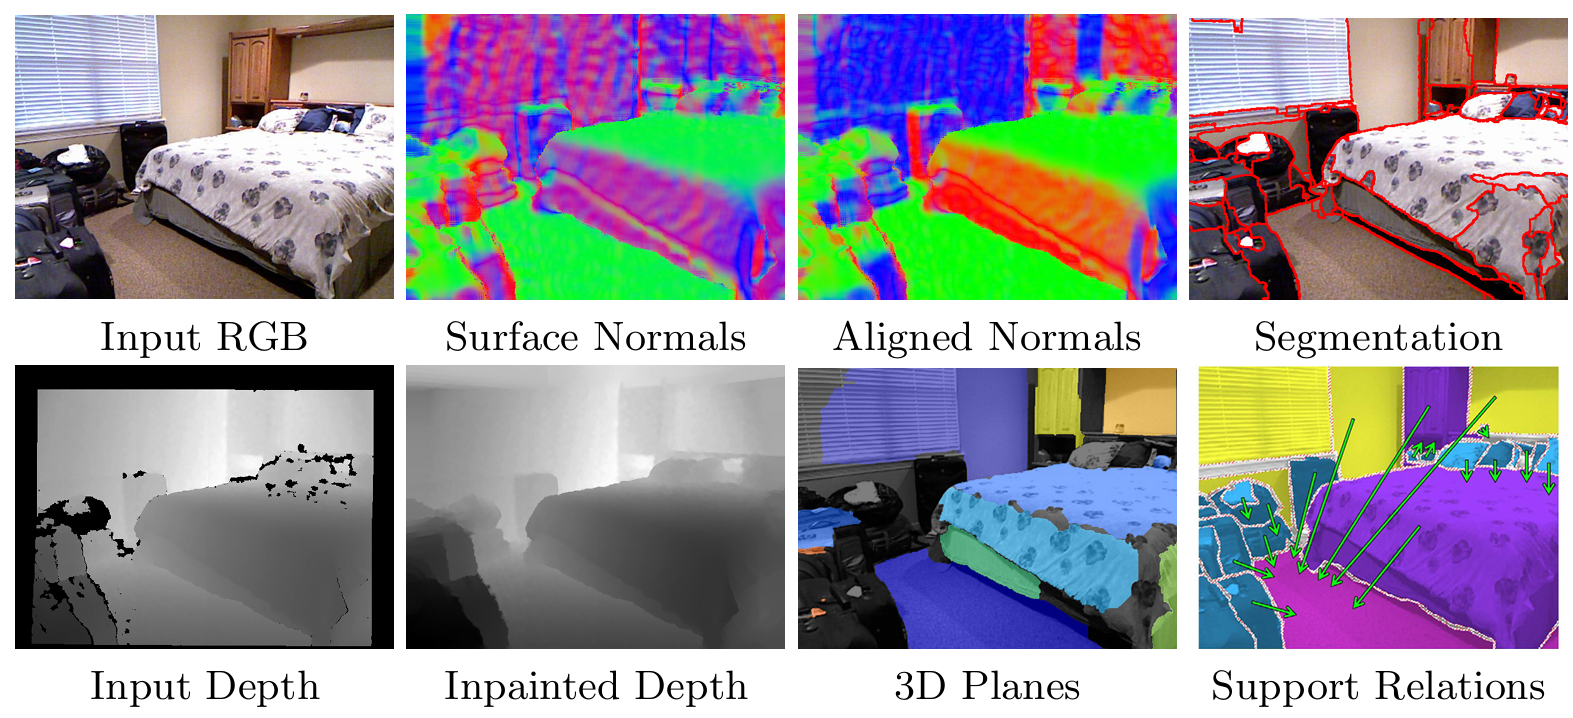
\includegraphics[width=\textwidth]{figs/nyuv2_example}
    \caption[Examples from NYUv2 dataset.]{
        Image and its annotations from NYUv2 paper \cite{NYUv2}.
        \label{fig:nyuv2_example}
    }
\end{figure}
%%%%%%%%%%%%%%%%%%%%%%%%%%%%%%%%%%%%%%%%%%

\subsection{NYUv2}
Many robotics and scene understanding applications require a physical parse of the scene into objects, surfaces, and their relation \cite{NYUv2}.
The NYUv2 dataset \cite{NYUv2} is a collection of 1449 annotated RGBD images from indoor environments of US commercial and residential buildings.
Depth is measured thanks to a Kinect sensor jointly capturing images with the RGB camera.
As it can be seen in figure \ref{fig:nyuv2_example}, provided geometry information about the scene is not just depth.
From the RGBD images are produced surface normal maps, segmentation, 3D planes and support relations through various estimation procedures.
For instance, for producing the surface normal map, to each pixel they fitted a plane, by least square minimization, to sampled surrounding pixels chosen based on a depth threshold.
NYUv2 dataset is frequently used for jointly learning multiple tasks for it provides various pixel-wise annotations.
As for the case of KITTI, here only the depth information will be relevant.

\section{Metrics and Evaluation}
\label{sec:metrics}

For quantifying the performance of depth estimation algorithms, various metrics are used in the literature.
Given the predicted depth map $\mathbf{Z}_{pred}$ of the model to evaluate and its corresponding groud-truth depth map $\mathbf{Z}_{gt}$, these metrics are defined as in table \ref{t:metrics}.

\begingroup
\renewcommand{\arraystretch}{2.}
\begin{table}
	%\begin{adjustwidth}{-0.2\textwidth}{-0.2\textwidth}
	\centering
	\resizebox{\textwidth}{!}{
	\begin{tabular}{r|l}
	Mean Absolute Relative Error (MARE) & $\frac{1}{\big| \mathbf{Z}^{*} \big|}\sum_{p \in \mathbf{Z}^{*}} \frac {\big| \mathbf{Z}^{*}(p) - \mathbf{Z}(p) \big|} {\mathbf{Z}^{*}(p)}$ \\
	Mean Squared Relative Error (MSRE) & $\frac{1}{\big| \mathbf{Z}^{*} \big|}\sum_{p \in \mathbf{Z}^{*}} \frac {\left( \mathbf{Z}^{*}(p) - \mathbf{Z}(p) \right)^{2}} {\mathbf{Z}^{*}(p)}$ \\
	Root Mean Squared Error (RMSE) & $\sqrt{
		\frac{1}{\big| \mathbf{Z}^{*} \big|}\sum_{p \in \mathbf{Z}^{*}} \left( \mathbf{Z}^{*}(p) - \mathbf{Z}(p) \right)^{2}
	}$ \\
	Root Mean Squared Log Error (RMSEL) & $\sqrt{
		\frac{1}{\big| \mathbf{Z}^{*} \big|}\sum_{p \in \mathbf{Z}^{*}} \left( log \, \mathbf{Z}^{*}(p) - log \, \mathbf{Z}(p) \right)^{2}
	}$ \\
	Accuracy with respect to a threshold ($\delta$) & $\frac{1}{\big| \mathbf{Z}^{*} \big|} \, \big| \{p \in \mathbf{Z}^{*} \, | \, \text{max}\{
		\frac{\mathbf{Z}^{*}(p)}{\mathbf{Z}(p)},
		\frac{\mathbf{Z}(p)}{\mathbf{Z}^{*}(p)}
	\} < \text{threshold} \} \big| $\\
	\end{tabular}
	}
%\end{adjustwidth}
\caption[Metrics and their definitions.]{
    Frequently used metrics in depth estimation literature.
    Common thresholds for $\delta$ are $1.25$, $1.25^{2}$ and $1.25^{3}$.
    \label{t:metrics}}
\end{table}
\endgroup

When computing them, not all pixels are considered and some processing is usually performed to mitigate certain problems.
For instance, LIDAR ground truth depth maps are often sparse, so $\mathbf{Z}^{*}(p)$ is not defined for all pixels $p \in \mathbf{Z}^{*}$.
Also, it is common practice to mask out reflective and transparent surfaces, as in \cite{Eigen}, for their ground truth labels are likely to be invalid.
Some authors also clamp the predicted depth maps \cite{Garg} to the ground truth depth range or mask out ground truth pixels corresponding to depth values above a certain threshold \cite{evalStudy}.
Moreover, models have diverse kind of outputs and output resolutions.
Some models output disparity maps, other depth maps.
Evaluating a given model on a certain dataset requires converting the model output format and output resolution to be compatible with the ones from the dataset ground truth data.
The resizing step involves interpolation, which can bias the model performance when the predictions are particularly small w.r.t. the ground truth data resolution \cite{evalStudy}.
Furthermore, not every dataset provides camera intrinsic parameters per image which are required for converting disparity maps to depth maps and some models are tuned on specific camera configurations.
This leads to another important matter: monocular depth estimation models do not have absolute geometric references to produce depth maps with the correct scale, unlike binocular depth estimation models.
This last issue particularly affects self-supervised models.
Eigen et al. \cite{Eigen} introduced a \textit{Scale-Invariant Error} upon which they also modeled their training loss.
They observed that correcting for the mean log depth of each prediction, substituting it with the corresponding ground truth one, leads to a 20\% relative improvement in performance.
Their \textit{Scale-Invariant Error} is invariant to scale in the sense that, by pixel-wise multiplying a prediction or a ground truth depth map for a positive value, the corresponding error remains unchanged.
\[
	\textit{Scale-Invariant Error} =
		\text{mean}_{p, q \in \mathbf{Z}^{*}}
		(
			( log \, \mathbf{Z}(p) - log \, \mathbf{Z}(q)) -
			( log \, \mathbf{Z}^{*}(p) - log \, \mathbf{Z}^{*}(q))
		)^{2}
\]

\begin{table}
	%\begin{adjustwidth}{-0.2\textwidth}{-0.2\textwidth}
	\centering
	\resizebox{\textwidth}{!}{
	\begin{tabular}{l|l|l|l|l|l|l|l|l}
		\emph{Method} & \emph{Year} & \emph{MARE} & \emph{MSRE} & \emph{RMSE} & \emph{RMSEL} & \emph{$\delta \, 1.25$} & \emph{$\delta \, 1.25^{2}$} & \emph{$\delta \, 1.25^{3}$} \\
		\hline
		Eigen et al. \cite{Eigen}                  & 2014 & 0.190 & 1.515 & 7.156 & 0.270 & 0.692 & 0.899 & 0.967 \\
		Garg et al. \cite{Garg}                    & 2016 & 0.169 & 1.080 & 5.104 & 0.273 & 0.740 & 0.904 & 0.962 \\
		MonoDepth \cite{MonoDepth}                 & 2017 & 0.097 & 0.896 & 5.093 & 0.176 & 0.879 & 0.962 & 0.986 \\
		SfMLearner \cite{SfMLearner}               & 2017 & 0.208 & 1.768 & 6.856 & 0.283 & 0.678 & 0.885 & 0.957 \\
		Cao et al. \cite{depth_as_classification}  & 2017 & 0.153 &   -   & 5.290 &   -   & 0.814 & 0.939 & 0.976 \\
		Fu et al. \cite{ordinal_regression}        & 2018 & 0.072 & 0.307 & 2.727 & 0.120 & 0.932 & 0.984 & 0.994 \\
		MonoDepth2 \cite{MonoDepth2}               & 2018 & 0.106 & 0.806 & 4.630 & 0.193 & 0.876 & 0.958 & 0.980 \\
		struct2depth \cite{struct2depth}           & 2018 & 0.108 & 0.825 & 4.750 & 0.186 & 0.873 & 0.957 & 0.982 \\
		vid2depth \cite{vid2depth}                 & 2018 & 0.151 & 0.949 & 4.383 & 0.227 & 0.802 & 0.935 & 0.974 \\
		FeatDepth \cite{FeatDepth}                 & 2020 & 0.099 & 0.697 & 4.427 & 0.184 & 0.889 & 0.963 & 0.982 \\
		denseViT \cite{denseViT}                   & 2021 & 0.062 &   -   & 2.573 & 0.092 & 0.959 & 0.995 & 0.999 \\
		AdaBins \cite{AdaBins}                     & 2021 & 0.058 & 0.190 & 2.360 & 0.088 & 0.964 & 0.995 & 0.999 \\
	\end{tabular}
}
%\end{adjustwidth}
	\caption[KITTI benchmarks.]{
		\textbf{KITTI} benchmarks.
		\label{t:kitti_benchmarks}
	}
\end{table}

In \cite{SfMLearner} Zhou et al. scale each prediction $\mathbf{Z}$ of their model by $\frac{\text{median}(\mathbf{Z}^{*})}{\text{median}(\mathbf{Z})}$, so to obtain an evaluation independent of scale also for the other metrics.
Godard et al. also follow this approach in \cite{MonoDepth2}, but they make the scaling factor equal across all images by taking the mean of all the median scales both for predictions and ground truth observations:
\[
	\frac{
		\text{mean}_{\mathbf{Z}^{*}} (\text{median} ( \mathbf{Z}^{*}))
	}{
		\text{mean}_{\mathbf{Z}} (\text{median} ( \mathbf{Z}))
	}
\]
They argue that: adapting the depth distribution with a scaling factor defined per image, hides large scale variations in the predicted depth maps, which is undesirable if one wants to apply the model to a sequence of images, in which there must be temporal consistency of the scales.
As discussed in \cite{evalStudy}, these processing steps affect in different ways the resulting metrics.
The same authors also observe that higher quantitative performance doesn't necessarily imply better qualitative appearance.
In \cite{monocular2024} it is noted that a specifically designed metric that satisfies the need of the depth estimation task has not been established yet.
Researchers in this field are still searching for new alternatives.

\vspace{0.5cm}

Benchmarks of many of the treated works are shown in table \ref{t:kitti_benchmarks} and \ref{t:NYUv2_benchmarks}.
Since the results come from disparate methods that worked in various depth estimation settings, there is not a monotonical temporal increase in performances.
Supervised \textit{metric} depth estimation works exhibit better performance indicator.
These are: \cite{Eigen}, \cite{Eigen2}, \cite{depth_as_classification}, \cite{ordinal_regression}, \cite{denseViT}, \cite{AdaBins}, \cite{Laina}, \cite{LocalBins}, \cite{ZoeDepth}.

\begin{table}
	%\begin{adjustwidth}{-0.2\textwidth}{-0.2\textwidth}
	\centering
	\resizebox{\textwidth}{!}{
	\begin{tabular}{c|c|c|c|c|c|c|c|c}
	\emph{Method} & \emph{Year} & \emph{MARE} & \emph{MSRE} & \emph{RMSE} & \emph{RMSEL} & \emph{$\delta \, 1.25$} & \emph{$\delta \, 1.25^{2}$} & \emph{$\delta \, 1.25^{3}$} \\
	\hline
	Eigen et al. \cite{Eigen}                      & 2014 & 0.215 & 0.212 & 0.907 & 0.285 & 0.611 & 0.887 & 0.971 \\
	Eigen et al. \cite{Eigen2}                     & 2015 & 0.158 & 0.121 & 0.641 & 0.214 & 0.769 & 0.950 & 0.988 \\
	Laina et al. \cite{Laina}                      & 2016 & 0.127 &   -   & 0.573 & 0.195 & 0.811 & 0.953 & 0.988 \\
	DIW \cite{DIW}                                 & 2016 & 0.360 & 0.460 & 1.130 & 0.390 &   -   &   -   &   -   \\
	Cao et al.   \cite{depth_as_classification}    & 2017 & 0.192 &   -   & 0.688 &   -   & 0.722 & 0.926 & 0.980 \\
	ReDWeb \cite{ReDWeb}                           & 2018 & 0.340 & 0.410 & 1.090 & 0.370 & 0.781 & 0.950 & 0.987 \\
	Fu et al. \cite{ordinal_regression}            & 2018 & 0.115 &   -   & 0.509 &   -   & 0.828 & 0.965 & 0.992 \\
	denseViT \cite{denseViT}                       & 2021 & 0.110 &   -   & 0.357 &   -   & 0.904 & 0.988 & 0.998 \\
	AdaBins \cite{AdaBins}                         & 2021 & 0.103 &   -   & 0.364 &   -   & 0.903 & 0.984 & 0.997 \\
	LocalBins \cite{LocalBins}                     & 2022 & 0.099 &   -   & 0.357 &   -   & 0.907 & 0.987 & 0.998 \\
	ZoeDepth \cite{ZoeDepth}                       & 2023 & 0.075 &   -   & 0.270 &   -   & 0.955 & 0.995 & 0.999 \\
	\end{tabular}
	}
%\end{adjustwidth}
	\caption[NYUv2 benchmarks.]{
		\textbf{NYUv2} benchmarks.
		\label{t:NYUv2_benchmarks}
	}
\end{table}

The worst performing models are the ones that come from \cite{DIW} and \cite{ReDWeb}.
In fact, they are \textit{relative} depth estimation models and these metrics are used to measure metric depth values.
The authors showed that, despite metric information was completely absent in the training phase, models managed to be at least comparable with metric models in terms of performance.
In relative depth estimation different metrics are employed for evaluation purposes.
A common one, found both in \cite{DIW} and \cite{ReDWeb}, is the Weighted Kinetic Disagreement Rate (WKDR).
I won't define it here, refer to \cite{Zoran} in which Zoran et al. firstly introduced it.

Self-supervised models place in the middle, but, depending on whether the supervision was on stereo data (that implicitly contain metric information) or monocular footage, there are observable differences.
\cite{Garg}, \cite{MonoDepth}, \cite{MonoDepth2}, \cite{struct2depth}, \cite{vid2depth}, \cite{FeatDepth}, \cite{SfMLearner} train models in a self-supervised manner.

\vspace{0.5cm}

The metrics defined in this section are the ones used by Eigen et al. in \cite{Eigen} for metric depth estimation on KITTI and NYUv2.
Their work was the first deep learning based approach to depth estimation and has been taken as a reference for a long time.
As this field evolved, there has been some change in how researchers evaluated their work.
This can be seen also dataset-wise!
Benchmarks on NYUv2 stopped reporting MSRE and RMSEL, using instead a log relative error.

The work of Ranftl et al. \cite{MiDas} started the zero-shot research line in depth estimation.
While the used metrics didn't change, the evaluation procedure did.
Models are trained on a dataset and the evaluation is run on a whole different dataset.
When doing this, researchers only report a pair of metrics, usually an error metric and an accuracy.
Fall into this category \cite{MiDas}, \cite{PatchFusion}, \cite{Marigold}, \cite{ZoeDepth}.